%%%%%%%%%%%%%%%%%%%%%%%%%%%%%%%%%%%%%%%%%
% University Assignment Title Page 
% LaTeX Template
% Version 1.0 (27/12/12)
%
% This template has been downloaded from:
% http://www.LaTeXTemplates.com
%
% Original author:
% WikiBooks (http://en.wikibooks.org/wiki/LaTeX/Title_Creation)
%
% License:
% CC BY-NC-SA 3.0 (http://creativecommons.org/licenses/by-nc-sa/3.0/)
%%%%%%%%%%%%%%%%%%%%%%%%%%%%%%%%%%%%%%%%%

% To display title in overleaf project overview
% \title{Machine Learning #11}

%-------------------------------------------------------
%	PACKAGES AND OTHER DOCUMENT CONFIGURATIONS
%-------------------------------------------------------

\documentclass[12pt]{article}
\usepackage[a4paper]{geometry}
\usepackage[english]{babel}
\usepackage[utf8x]{inputenc}
\usepackage{amsmath}
\usepackage{graphicx}
\usepackage{subcaption}
\usepackage[colorinlistoftodos]{todonotes}
\usepackage{tikz}

\begin{document}

\def\layersep{2.5cm}

\begin{titlepage}

% Defines a new command for the horizontal lines, change thickness here
\newcommand{\HRule}{\rule{\linewidth}{0.4mm}} 

% Center everything on the page
\center 
 
%-------------------------------------------------------
%	HEADING SECTIONS
%-------------------------------------------------------

\textsc{\LARGE Jacobs University}\\[1.5cm] % University
\textsc{\Large Machine Learning}\\[0.5cm] % Major
\textsc{\large Exercise Sheet 11}\\[0.5cm] % Minor

%-------------------------------------------------------
%	TITLE SECTION
%-------------------------------------------------------

\HRule \\[0.4cm]
{ \huge \bfseries Solving the XOR function using an MLP}\\[0.4cm] % Title of your document
\HRule \\[1.5cm]
 
%-------------------------------------------------------
%	AUTHOR SECTION
%-------------------------------------------------------

% \begin{minipage}{0.4\textwidth}
% \begin{flushleft} \large
% \emph{Authors:}\\
% Alex \textsc{Maiereanu}\\
% Tudor \textsc{Maiereanu}\\
% Steven \textsc{Abreu}
% \end{flushleft}
% \end{minipage}
% ~
% \begin{minipage}{0.4\textwidth}
% \begin{flushright} \large
% \emph{Supervisor:} \\
% Dr. Herbert \textsc{Jaeger}\\
% \ \\
% \ 
% \end{flushright}
% \end{minipage}\\[2cm]

\Large \emph{Authors:}\\
Steven \textsc{Abreu}\\
Alex \textsc{Maiereanu}\\
Tudor \textsc{Maiereanu}\\[3cm] % Your name

%-------------------------------------------------------
%	DATE SECTION
%-------------------------------------------------------

{\large \today}\\[2cm]

%-------------------------------------------------------
%	LOGO SECTION
%-------------------------------------------------------

% \includegraphics{logo.png}\\[1cm]
 
%-------------------------------------------------------

\vfill

\end{titlepage}


%\begin{abstract}
%Your abstract.
%\end{abstract}

\section{Task}

\textbf{Outline.} Implement an MLP with a single hidden layer from scratch and train it on a classical historical challenge problem, the XOR function. You can earn valuable bonus points by going beyond this basic task, see end of this task sheet.\\

\noindent
\textbf{Data and learning task.} The task is to train an MLP on the exclusive-OR function $XOR: \{0, 1\}^2 \rightarrow \{0, 1\}$ given by 
\begin{equation}
	XOR(x,y) = \begin{cases}
		0 & \text{if } x = y\\
		1 & \text{if } x \neq y
	\end{cases}
\end{equation} 
with an MLP that has 2 input units and one output unit. The training data consists of the four input-output pairs that define the XOR function. Note that this is a noise-free deterministic task and the function is completely covered by the training data. There are no "new" test data, hence training and test error coincide. This means that all the over/underfitting problems are a non-issue here – all you have to aim for is a low training error.\\

\noindent
\textbf{Suggested network structure.} For this problem an MLP with a single hidden layer that has 2 units suffices. Also include bias units in the input and the hidden layer, as in Figure 25 in the lecture notes. I suggest you use the logistic sigmoid in the hidden layer, simply because its derivative is described in the lecture notes.\\

\noindent
\textbf{Learning goal.} The purpose of this exercise is not so much to solve the XOR learning problem, but to become a close acquaintance of the most widely used learning algorithm im ML, backprop – and shake hands with history. You can basically just put the formulas 53, 55, 59, 61, 63 in the lecture notes into program code, which is not in itself difficult, but error-prone (you will presumably be hit by that sad fact), and on that way you have to inspect and understand each of those little formulas, which is what this exercise aims to achieve.\\

\noindent
\textbf{Detailed instructions.} Implement an MLP with the structure outlined above, and implement backprop to compute the error gradients. I suggest to use the quadratic loss with no regularizer. Initialize your MLP with small random weights. After each epoch, compute the mean training squared error.\\
At any stage during training, your MLP will give output values that are real numbers, not clean 0 or 1 values. If you postprocess the MLP outputs by thresholding at 0.5 (postprocessed output = 1 if MLP output $> 0.5$, else = 0) your MLP turns into a Boolean function. After some training epochs this Boolean function will be the XOR. You may stop at that point and be satisfied, or you may continue training to make the MLP output come closer and closer to the precise 0-1-values.\\

\noindent
\textbf{Deliverable.} A typeset report which documents your learning set-up (initialization, learning rate) and shows a graphics of the learning curve, that is a plot of the mean training error vs. the epoch number. Target size: 1.5 pages, excluding graphics. Plus, your code. It should be a self-contained single script (Matlab or Python) which does the complete network creation, initialization, learning and plotting.\\

\noindent
\textbf{Grading.} A nicely done report and functioning code will give 100\%.\\

\noindent
\textbf{Bonus points} (max 5) are awarded for work that goes beyond the deliverable sketched above. Bonus points will be added undiluted to the final course grade, that is a bonus of 5 pts will, for example, raise a course grade from 85\% to 90\%.\\
Possible extensions for harvesting bonus points:
\begin{itemize}
	\item Instead of the Boolean XOR, train a continuous version of the same problem, namely a function $f: [-1, 1]^2 \rightarrow {0,1}$, defined by $f(x, y) = sign(xy)$. Display the performance of your final MLP by a nice 2-dim surface graphic.
	\item Try to train more complex Boolean functions. A classical teaser is the parity function: $P: {0,1}^n \rightarrow {0,1}$ given by:
		\begin{equation}
			P(x) = \begin{cases}
				1 & \text{if the number of 1's in the Boolean vector $x$ is even}\\
				0 & \text{otherwise}
			\end{cases}
		\end{equation}
		When $n$ grows, this quickly becomes a (very) difficult learning task.
	\item Train an MLP classifier on our digits dataset. This is a much more demanding task because now you have to fight with the bias-variance dilemma and find a way to prevent overfitting (suggestion: use a large enough MLP with 2 hidden layers and use early stopping for regularization). If you can push the final classification test error (on the standard test data consisting of the second 100 images per class) below 3\%, you can feel very satisfied. The best ML methods reported in the literature achieve about 1.8\% test error, but they employ combinations of several methods, not just a single MLP.
\end{itemize}

%\clearpage
%\textbf{Summary}. Implement an MLP with:
%\begin{itemize}
%	\item 1 hidden layer with 2 units. Include bias units in input and hidden layers.
%	\item Logistic sigmoid in the hidden layer.
%	\item Back-propagation and gradient descent.
%	\item Quadratic loss and no regularizer.
%	\item Initialized with small random weights.
%	\item Test data same as training data: $\{(0,0,0), (1,1,0), (1,0,1), (0,1,0)\}$.
%	\item After each epoch, compute the MSE$^{train}$.
%	\item Threshold the output by rounding to either 0 or 1.
%	\item Train until XOR function implemented (maybe continue until more accurate and close to precise 0-1-values).
%\end{itemize}

\clearpage
\section{Solving the XOR function with an MLP}

We used an MLP with one hidden layer that uses one neuron for the input layer (plus one bias neuron), two neurons for the hidden layer (plus one bias neuron) and one output neuron, as illustrated below:
\begin{center}
\begin{tikzpicture}[shorten >=1pt,->,draw=black!50, node distance=\layersep]
    \tikzstyle{every pin edge}=[<-,shorten <=1pt]
    \tikzstyle{neuron}=[circle,fill=black!25,minimum size=17pt,inner sep=0pt]
    \tikzstyle{input neuron}=[neuron, fill=green!50];
    \tikzstyle{output neuron}=[neuron, fill=red!50];
    \tikzstyle{hidden neuron}=[neuron, fill=blue!50];
    \tikzstyle{annot} = [text width=4em, text centered]

    % Draw the input layer nodes
    \foreach \name / \y in {1,...,1}
    % This is the same as writing \foreach \name / \y in {1/1,2/2,3/3,4/4}
        \node[input neuron, pin=left:Input \#\y] (I-\name) at (0,-1) {};
    \node[input neuron, pin=left: Bias] (I-2) at (0,-2) {};

    % Draw the hidden layer nodes
    \foreach \name / \y in {1,...,3}
        \path[yshift=0.5cm]
            node[hidden neuron] (H-\name) at (\layersep,-\y cm) {};
    \node[hidden neuron, pin=left: Bias] (H-3) at (\layersep,-2.5 cm) {};

    % Draw the output layer node
    \node[output neuron,pin={[pin edge={->}]right:Output}, right of=H-1] (O) {};

    % Connect every node in the input layer with every node in the
    % hidden layer.
    \foreach \source in {1,...,2}
        \foreach \dest in {1,...,2}
            \path (I-\source) edge (H-\dest);

    % Connect every node in the hidden layer with the output layer
    \foreach \source in {1,...,3}
        \path (H-\source) edge (O);

    % Annotate the layers
    \node[annot,above of=H-1, node distance=1cm] (hl) {Hidden layer};
    \node[annot,left of=hl] {Input layer};
    \node[annot,right of=hl] {Output layer};
\end{tikzpicture}
\end{center}

Our MLP uses the Sigmoid function in the hidden layer.\\
For training, we used the backpropagation algorithm. For our errors, we used quadratic loss with no regularizer. Our training data is the same as our testing data, which is: $\{(0,0), (1,1), (1,0), (0,1)\}$ with the targets: $\{0,0,1,1\}$. \\
We initialized our neural network with small random weights, $w_{ij} \in [-1,1]$. In each epoch of the training procedure, we go through the training data once. We used the learning rate $\lambda = 0.1$. \\
For 10.000 epochs, we get the following error plot:

\begin{figure}[h!]
	\centering
	\begin{subfigure}{.49\linewidth}
	  \centering
	  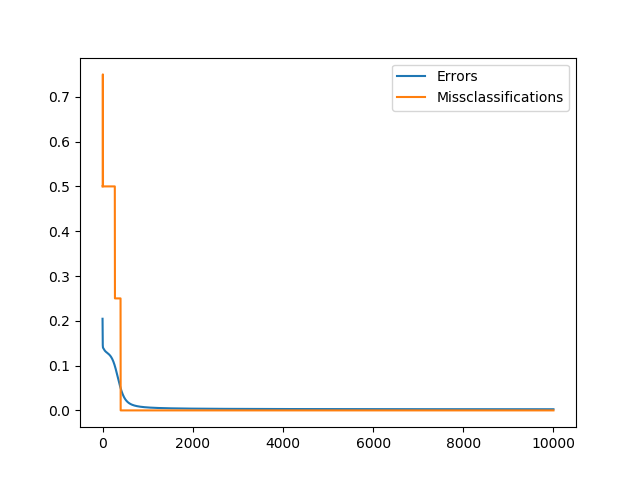
\includegraphics[width=\linewidth]{img/xor10000.png}
	  \caption{10.000 epochs}
	  \label{fig:xor10000}
	\end{subfigure}
	\begin{subfigure}{.49\linewidth}
	  \centering
	  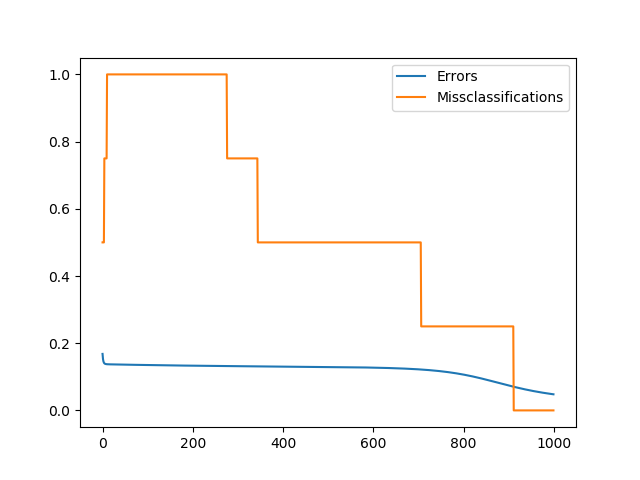
\includegraphics[width=\linewidth]{img/xor1000.png}
	  \caption{1.000 epochs}
	  \label{fig:xor1000}
	\end{subfigure}
	\caption{Plot of MSE and MISS for XOR MLP}
	\label{fig:test}
\end{figure}

\noindent
From the graph, it is easy to see that after around 1.000 epochs, we have no more classifications, but we can continue training in order to further reduce the mean squared error. 

\section{Training an MLP for the Sign function}

We want to train our MLP to recognize the function:
\begin{equation}
	sign: [0,1]^2 \rightarrow \{0,1\}
\end{equation}
\begin{equation}
	sign(x,y) = \begin{cases}
		0 & \text{if } xy < 0\\
		1 & \text{otherwise}
	\end{cases}
\end{equation}

\noindent
We used the following structure for our neural network:

\begin{center}
\begin{tikzpicture}[shorten >=1pt,->,draw=black!50, node distance=\layersep]
    \tikzstyle{every pin edge}=[<-,shorten <=1pt]
    \tikzstyle{neuron}=[circle,fill=black!25,minimum size=17pt,inner sep=0pt]
    \tikzstyle{input neuron}=[neuron, fill=green!50];
    \tikzstyle{output neuron}=[neuron, fill=red!50];
    \tikzstyle{hidden neuron}=[neuron, fill=blue!50];
    \tikzstyle{annot} = [text width=4em, text centered]

    % Draw the input layer nodes
    \foreach \name / \y in {1,...,2}
    % This is the same as writing \foreach \name / \y in {1/1,2/2,3/3,4/4}
        \node[input neuron, pin=left:Input \#\y] (I-\name) at (0,-\y) {};
    \node[input neuron, pin=left: Bias] (I-3) at (0,-3) {};

    % Draw the hidden layer nodes
    \foreach \name / \y in {1,...,4}
        \path[yshift=0.5cm]
            node[hidden neuron] (H-\name) at (\layersep,-\y cm) {};
    \node[hidden neuron, pin=left: Bias] (H-5) at (\layersep,-4.5 cm) {};

    % Draw the output layer node
    \node[output neuron,pin={[pin edge={->}]right:Output}, right of=H-1] (O) {};

    % Connect every node in the input layer with every node in the
    % hidden layer.
    \foreach \source in {1,...,3}
        \foreach \dest in {1,...,4}
            \path (I-\source) edge (H-\dest);

    % Connect every node in the hidden layer with the output layer
    \foreach \source in {1,...,5}
        \path (H-\source) edge (O);

    % Annotate the layers
    \node[annot,above of=H-1, node distance=1cm] (hl) {Hidden layer};
    \node[annot,left of=hl] {Input layer};
    \node[annot,right of=hl] {Output layer};
\end{tikzpicture}
\end{center}

\noindent
Aside from additional input and hidden units, we left the MLP setup unchanged from the XOR MLP. We generated training patterns randomly in every epoch and generated random patterns for testing as well. \\
Using a 3D scatter plot, we visualized the misclassifications by marking correctly classified patterns in blue and wrongly classified patterns in red. We decided to use 1.000 epochs (with 1.000 training patterns each, thus a total of 1.000.000 training patterns). The following figure compares the performance of our MLP using either 4 hidden neurons or 10. \\
It is very obvious that 10 hidden neurons give us a much clearer classification with fewer misclassifications. 

\begin{figure}[h!]
	\centering
	\begin{subfigure}{.49\linewidth}
	  \centering
	  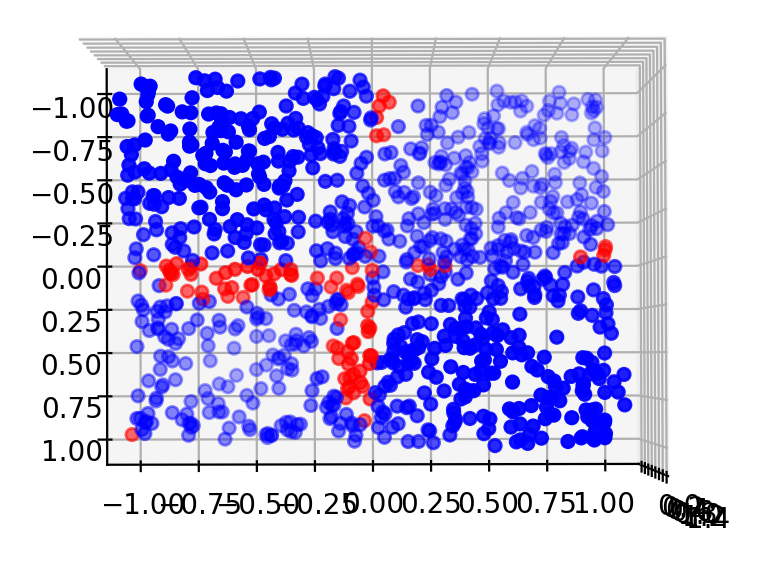
\includegraphics[width=\linewidth]{img/sign1M4.png}
	  \caption{Using 4 hidden neurons}
	  \label{fig:sign4}
	\end{subfigure}
	\begin{subfigure}{.49\linewidth}
	  \centering
	  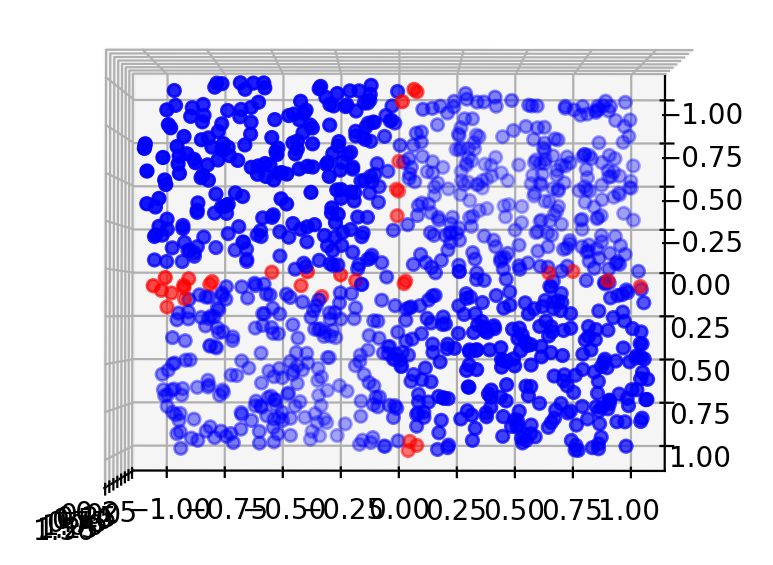
\includegraphics[width=\linewidth]{img/sign1M10.png}
	  \caption{Using 10 hidden neurons}
	  \label{fig:sign10}
	\end{subfigure}
	\caption{Plot of MSE and MISS for XOR MLP}
	\label{fig:test}
\end{figure}

\begin{figure}[h!]
	\centering
	\begin{subfigure}{.49\linewidth}
	  \centering
	  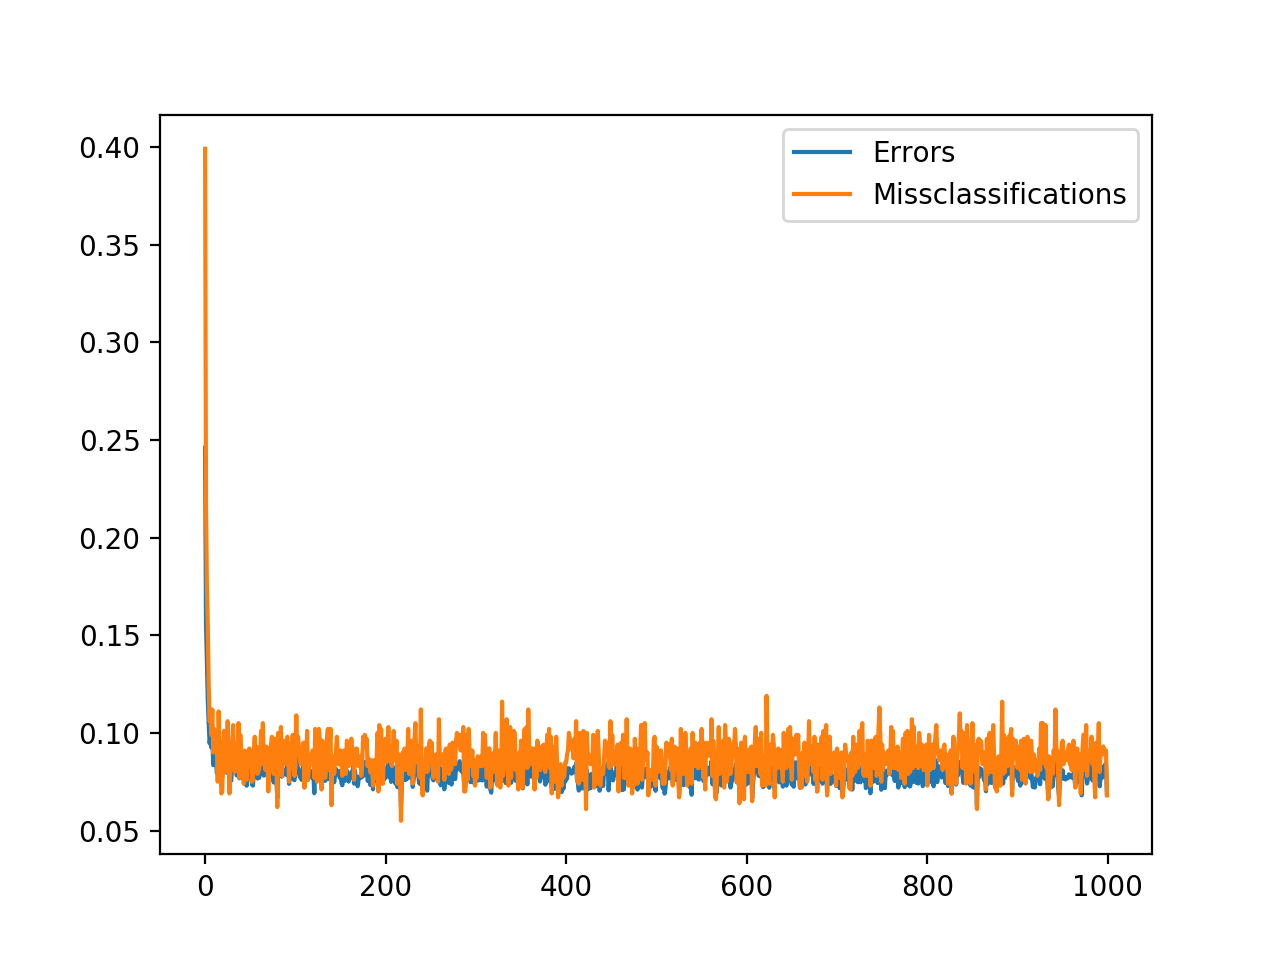
\includegraphics[width=\linewidth]{img/sign1M4E.png}
	  \caption{Using 4 hidden neurons}
	  \label{fig:sign4}
	\end{subfigure}
	\begin{subfigure}{.49\linewidth}
	  \centering
	  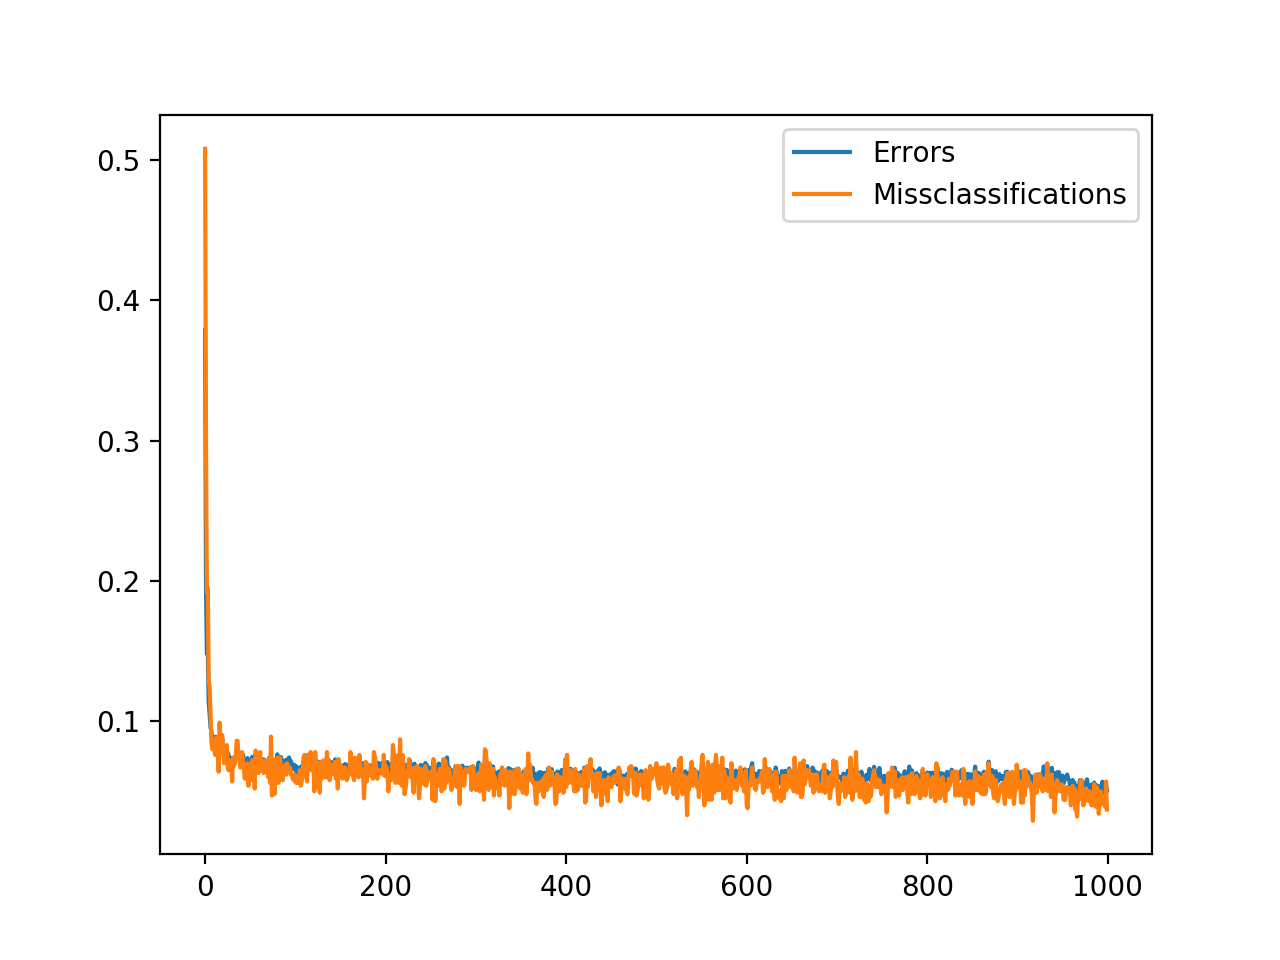
\includegraphics[width=\linewidth]{img/sign1M10E.png}
	  \caption{Using 10 hidden neurons}
	  \label{fig:sign10}
	\end{subfigure}
	\caption{Error plot of MSE and MISS for XOR MLP}
	\label{fig:test}
\end{figure}

\clearpage

\section{Training an MLP for Digit Classification}


% Margin comments
% Comments can be added to the margins of the document using the \todo{Here's a comment in the margin!} todo command, as shown in the example on the right. You can also add inline comments too:

% Inline comments
% \todo[inline, color=green!40]{This is an inline comment.}

% Referencing tables and figures
% Use the table and tabular commands for basic tables --- see Table~\ref{tab:widgets}, for example. You can upload a figure (JPEG, PNG or PDF) using the files menu. To include it in your document, use the includegraphics command as in the code for Figure~\ref{fig:frog} below.

%% Typesetting a table
% \begin{table}
% \centering
% \begin{tabular}{l|r}
% Item & Quantity \\\hline
% Widgets & 42 \\
% Gadgets & 13
% \end{tabular}
% \caption{\label{tab:widgets}An example table.}
% \end{table}

\end{document}